
\begin{figure}[h!]
    \centering
    \caption{Estimates of the effect of the minimum wage on rents, stacked sample including
             leads and lags}
    \label{fig:dynamic_stacked}

    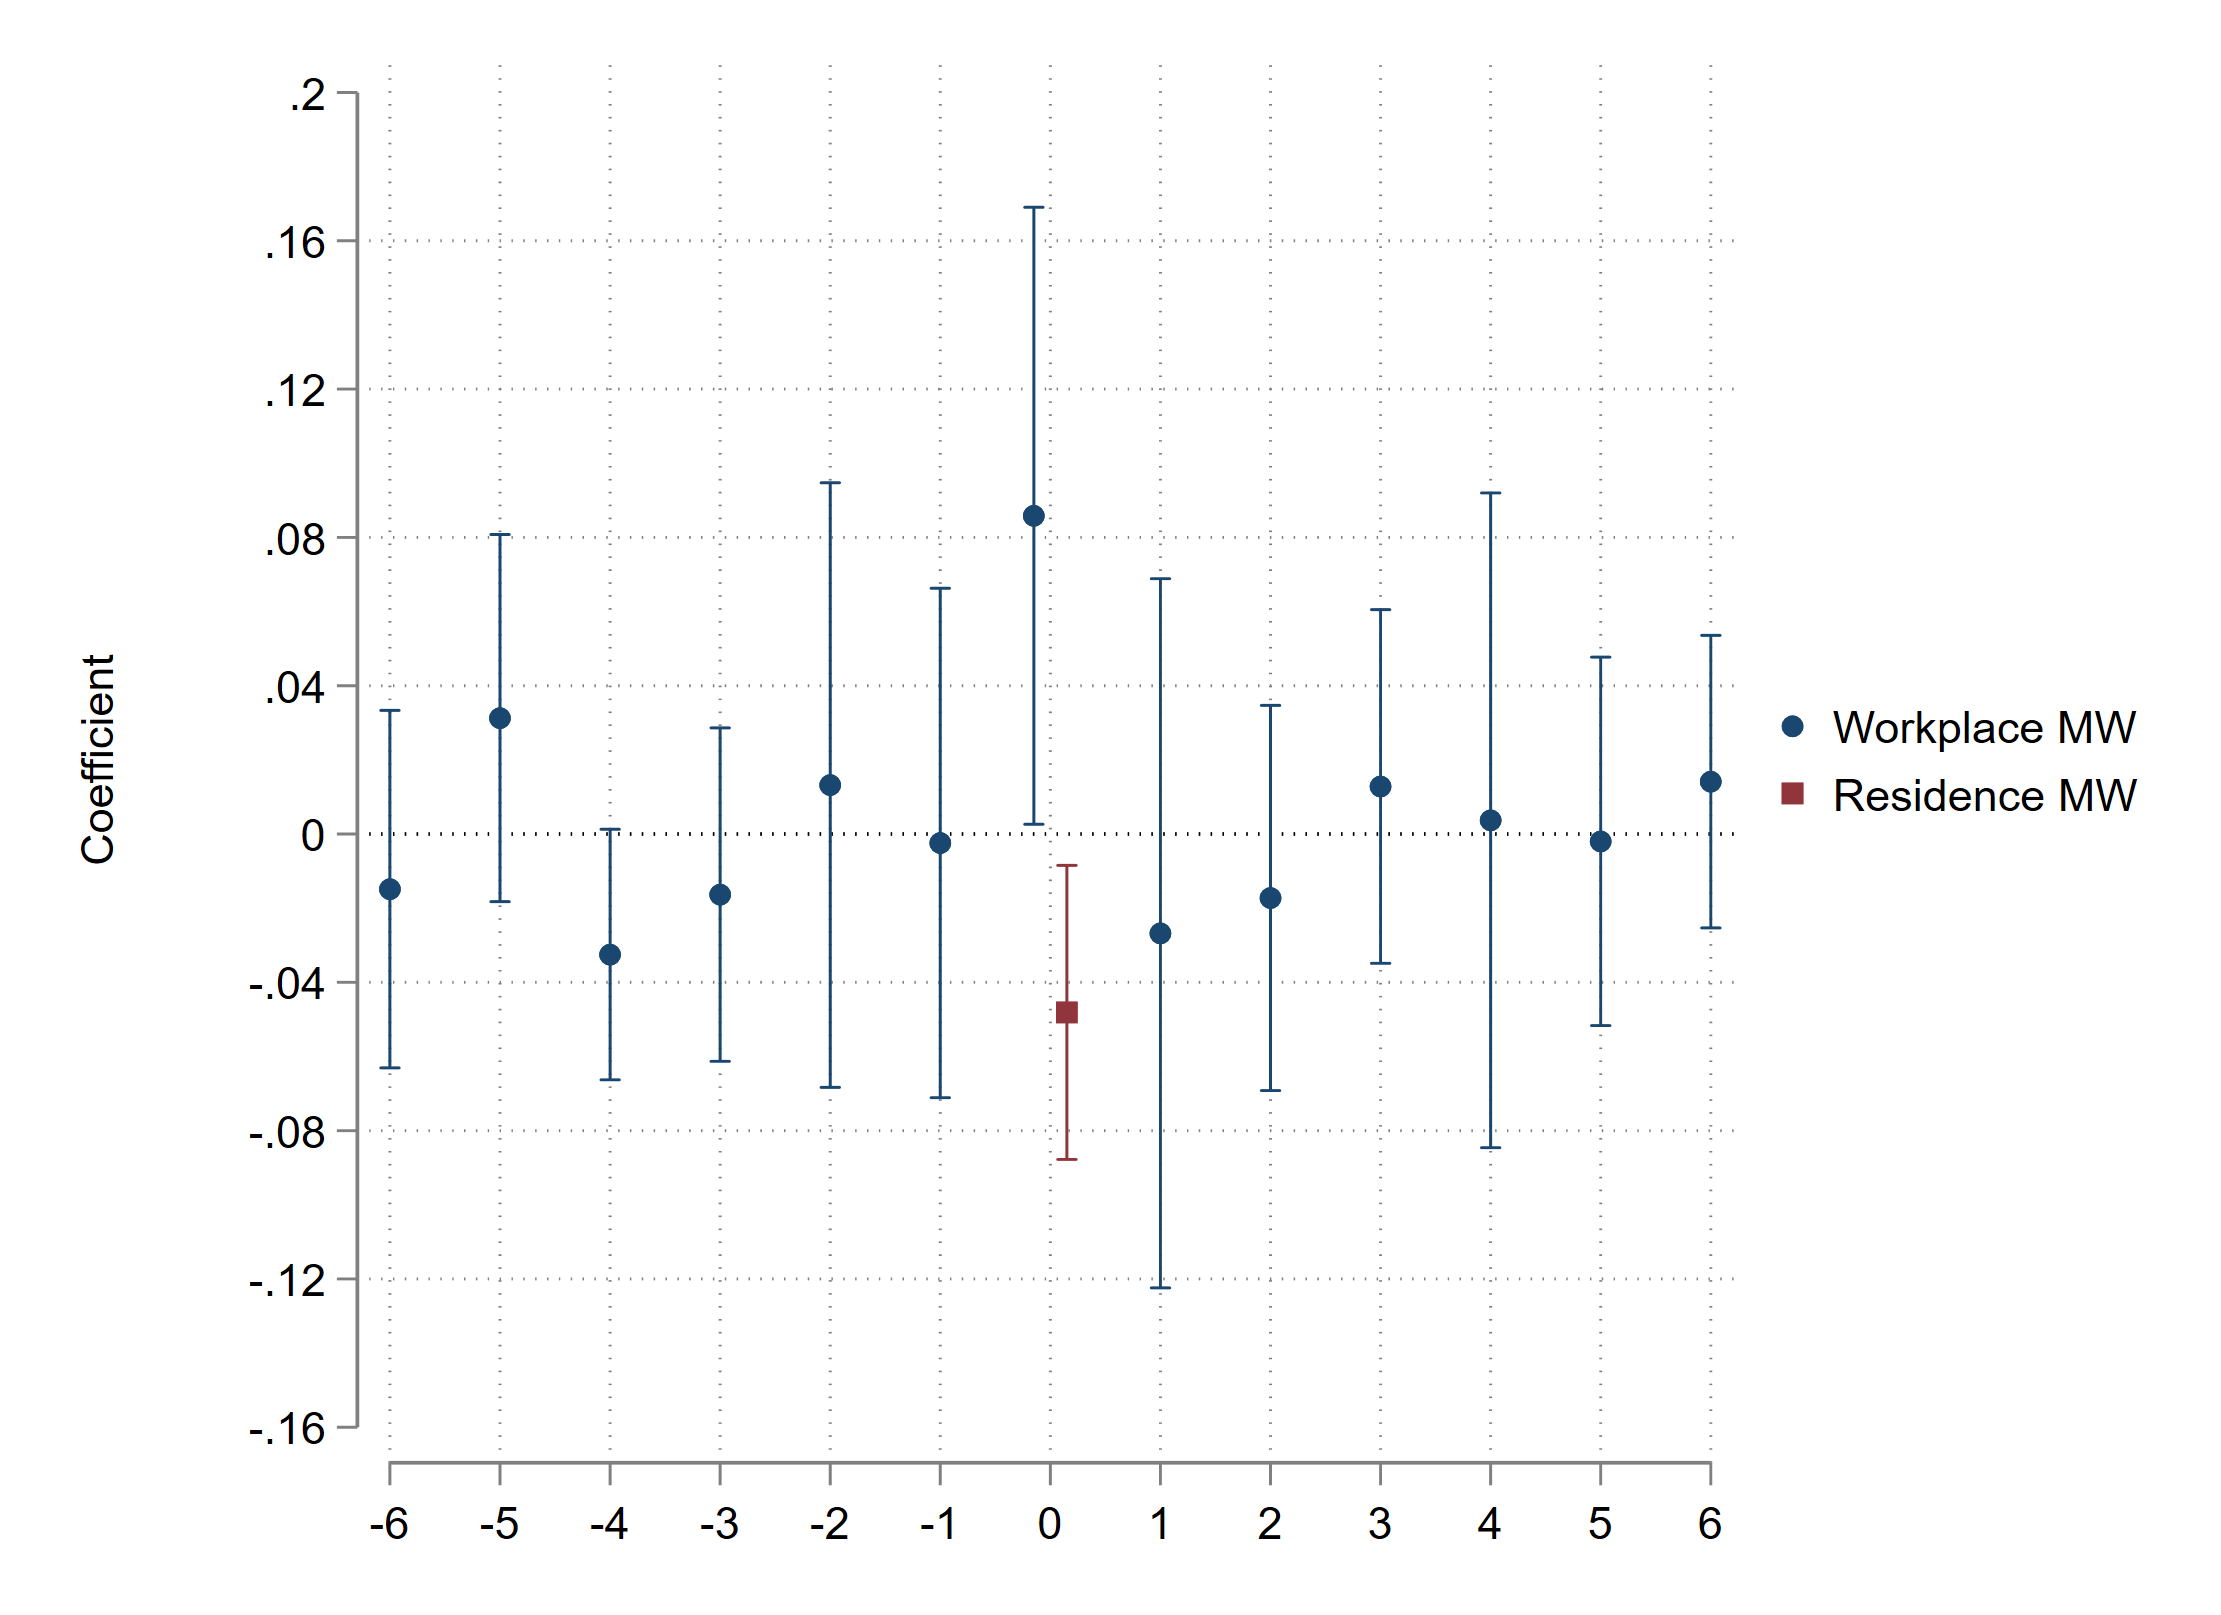
\includegraphics[width = 0.75\textwidth]{fd_stacked/output/fd_mw_wkp_only_dynamic_w6}

    \begin{minipage}{.95\textwidth} \footnotesize
        \vspace{3mm}
        Notes:
        Data are from Zillow,
        the MW panel described in Section \ref{sec:data_mw_panel},
        LODES origin-destination statistics,
        and the QCEW.
        The figure mimics estimates in Figure \ref{fig:dynamic_baseline} 
        using a ``stacked'' sample.
        We construct the sample as explained in Online Appendix Table 
        \ref{tab:stacked_w6}.
        95\% pointwise confidence intervals are obtained from standard errors 
        clustered at the state level.
    \end{minipage}
\end{figure}
